
  % !TeX root = RJwrapper.tex
\title{Working with CRSP/COMPUSTAT in R: Reproducible Empirical Asset Pricing}
\author{by Majeed Simaan}

\maketitle

\abstract{
It is common to come across SAS or Stata manuals while working on academic empirical finance research. Nonetheless, given the popularity of open-source programming languages such as  R, there are fewer resources  in R covering popular databases such as CRSP and COMPUSTAT. The aim of this article is to bridge the gap and illustrate how to leverage R in working with both datasets. As an application, we illustrate how to form size-value portfolios with respect to \cite{fama1993common} and study the sensitivity of the results with respect to different inputs. Ultimately, the purpose of the article is to advocate  reproducible finance research and contribute to the recent idea of  ``Open Source Cross-Sectional Asset Pricing'', proposed by \citet{chen2020open}.
}



\hypertarget{overview}{%
\section{Overview}\label{overview}} 
Typically the \cite{CRSP} and \cite{COMPUSTAT} databases are viewed as the cornerstones of academic empirical finance research. The former corresponds to security-related information for publicly listed companies, such as closing prices and returns. The latter covers financial statements disclosed  by public firms, such as income statement, balance sheet, and cash-flow related items. We begin our discussion by demonstrating how to  clean, manipulate, and merge both datasets.  After doing so, we conduct the main analysis  from the perspective of empirical asset pricing research  based on  \cite{fama1993common}. 

The undertaken analysis constitutes  a typical portfolio formation procedure to investigate how investors are compensated for taking certain types of risk/style. 
 By grouping firms (stocks) with respect to pre-specified attributes, 
 the researcher can study the implications of these characteristics (risks) in association with  future returns. Such analysis is known as the cross-section of expected return
 (see, e.g., \cite{harvey2016and})  since the relationship is investigated on the firm/portfolio level. Consistent with \cite{harvey2016and}, we find that the results of the cross-section of expected returns are sensitive to the research design. In particular, the exclusion of small stocks in the sample has a significant economic impact. Small stocks tend to trade less frequently and to be less liquid. Hence, in order to better understand the cross-section of expected returns, one needs to take into consideration the underlying limits of arbitrage facing investors \citep{li2014limits}. 


We hope this article would further contribute to reproducible finance research and to our understandings of the cross-sectional of expected returns. 
  The article proceeds as follows. In Section \ref{data}, we discuss how to load each dataset along with the pre-analysis needed in order to merge the data altogether. Section \ref{forming-size-and-bm-portfolios} is devoted to the replication of \cite{fama1993common}'s size and value premiums. The analysis is conducted using raw and risk-adjusted returns. Section \ref{rendering-results} then proceeds to investigate the sensitivity of the cross-section  of returns with respect to the research design. Finally, Section \ref{concluding-remarks} concludes.



\hypertarget{data}{%
\section{Data}\label{data}}

The discussion assumes that the user has already downloaded the CRSP and
the COMPUSTAT datasets in two separate files, both in csv formats.\footnote{Note that users can work with the database directly using the WRDS API.} The article will rely on different  libraries to perform the analysis. The core packages of
interest are  \CRANpkg{data.table} \citep{data.table} and \CRANpkg{lubridate} \citep{lubridate}. 
We also refer to \CRANpkg{ggplot2} \citep{ggplot2} to produce figures and \CRANpkg{parallel} \citep{parallel} to perform parallel processing. 
In a few cases, we refer to \CRANpkg{plyr} \citep{plyr} and \CRANpkg{dplyr}  \citep{dplyr}  for additional data manipulation. Nonetheless, the main analysis is conducted in the
\pkg{data.table} environment.
%\footnote{We are grateful to Matt Dowle and Arun Srinivasan for \pkg{data.table} and the DataCamp course ``Data
%Manipulation with data.table in R''.}

\begin{Schunk}
\begin{Sinput}
library(data.table)
library(lubridate)
library(ggplot2)
library(plyr)
library(parallel)
rm(list = ls())
\end{Sinput}
\end{Schunk}

\hypertarget{crsp}{%
\subsection{CRSP}\label{crsp}}

While there are a lot of pros to working \pkg{data.table}, one good
functionality is the option that allows the user to easily specify a
subset of variables while reading the whole data. Mostly, after
downloading the full dataset, we focus on a subset of variables of
interest. 
{\color{black}
We refer to its main function  \code{fread}, rather than the base command \code{read.csv}. The \code{fread} is similar to the base command; however, it provides faster and more convenient data manipulation. It is highly relevant when it comes to large data. Additionally, it allows users to easily utilize multi-threads using the  \code{nThread} argument.
}

\begin{Schunk}
\begin{Sinput}
file.i <- "CRSP_1960_2019.csv"
select.var <- c("PERMCO","date","COMNAM","SHROUT","SHRCD","DLRET",
                "DLSTCD","DLPDT","EXCHCD","RET","PRC","CUSIP")
DT  <- fread(file.i,select = select.var)
\end{Sinput}
\end{Schunk}
The above commands load the monthly CRSP dataset with pre-specified
variables. Those are the permanent identifier of the security
(\code{PERMCO}), date, shares outstanding in thousands
(\code{SHROUT}), share code (\code{SHRCD}), exchange code
(\code{EXCHCD}), security return \code{RET}, price \code{PRC}, and
the \code{CUSIP} identifier. Note that the CUSIP is the key link
between the CRSP and COMPUSTAT data. Additionally, we consider
delisting-related variables denoted by \code{DL}, which are discussed later.

\hypertarget{filters-and-cleaning}{%
\subsubsection{Filters and Cleaning}\label{filters-and-cleaning}}

After loading the data, we perform a few filters and cleaning procedures.
In particular, we keep common shares, those with 10 or 11 codes. We drop
missing values for prices. There are also certain flags for prices
denoted by -44, -55, -66, -77, -88, and -99. We drop these from the data
as well. Additionally, we keep securities listed on major exchanges
(NYSE, AMEX, or NASDAQ). Given these filters, we compute the market cap
for each stock-month in the data.

\begin{Schunk}
\begin{Sinput}
DT <- DT[DT$SHRCD %in% 10:11,]
DT <- DT[!is.na(DT$PRC),]
DT <- DT[!DT$PRC %in% (-(4:9)*11),]
DT$RET <- as.numeric(DT$RET)
DT <- DT[!is.na(DT$RET),]
DT$PRC <- abs(DT$PRC)
DT$MKTCAP <- DT$PRC*DT$SHROUT
DT <- DT[DT$EXCHCD %in% 1:3,]
\end{Sinput}
\end{Schunk}

There may be duplicates in the data depending on the identifier of
interest. To control for this, consider the following commands:

\begin{Schunk}
\begin{Sinput}
DT <- unique(DT)
DT <- DT[order(DT$PERMCO,DT$date),]
DT[ , `:=`( duplicate_N = .N   ) , by= list(PERMCO,date)]
table(DT$duplicate_N)/nrow(DT)*100
\end{Sinput}
\begin{Soutput}
#>            1            2            3            4            6            7 
#> 98.014830993  1.902150108  0.044272559  0.018337003  0.010738451  0.009670885
\end{Soutput}
\end{Schunk} %$
Note that the \code{:=} command creates a new variable to the already
existing \pkg{data.table}, where \code{.N} denotes the data length.
By grouping the data based on the stock identifier and month, we can
count whether there are multiple observations within each case. As we
observe from the above table, about 2\% of the observations are
duplicates, i.e., multiple observations for the same stock-month. For
instance, the table below illustrates the case in which we have 7
duplicates:

\begin{Schunk}
\begin{Sinput}
head(DT[DT$duplicate_N == 7,],7)
\end{Sinput}
\begin{Soutput}
#>    PERMCO     date                     COMNAM SHROUT SHRCD DLRET DLSTCD DLPDT
#> 1:  54311 20160531 LIBERTY MEDIA CORP 3RD NEW  25569    11           NA    NA
#> 2:  54311 20160531 LIBERTY MEDIA CORP 3RD NEW  55684    11           NA    NA
#> 3:  54311 20160531 LIBERTY MEDIA CORP 3RD NEW  10228    11           NA    NA
#> 4:  54311 20160531 LIBERTY MEDIA CORP 3RD NEW  22284    11           NA    NA
#> 5:  54311 20160531 LIBERTY MEDIA CORP 3RD NEW 102277    11           NA    NA
#> 6:  54311 20160531 LIBERTY MEDIA CORP 3RD NEW   9871    11           NA    NA
#> 7:  54311 20160531 LIBERTY MEDIA CORP 3RD NEW 222735    11           NA    NA
#>    EXCHCD       RET   PRC    CUSIP    MKTCAP duplicate_N
#> 1:      3  0.064481 19.48 53122987  498084.1           7
#> 2:      3  0.052778 18.95 53122985 1055211.8           7
#> 3:      3  0.081873 15.56 53122970  159147.7           7
#> 4:      3  0.095723 15.00 53122988  334260.0           7
#> 5:      3 -0.026854 31.89 53122940 3261613.5           7
#> 6:      3 -0.026292 32.59 53122950  321695.9           7
#> 7:      3 -0.017801 31.45 53122960 7005015.8           7
\end{Soutput}
\end{Schunk} %$
Note that the duplicates arise due to different CUSIP identifiers. Since
we are planning to link the data with the COMPUSTAT using CUSIP, we
check whether there are duplicates for the same CUSIP-month:
\begin{Schunk}
\begin{Sinput}
DT[ , `:=`( duplicate_N = .N   ) , by= list(CUSIP,date)]
table(DT$duplicate_N)/nrow(DT)*100
\end{Sinput}
\begin{Soutput}
#>   1 
#> 100
\end{Soutput}
\begin{Sinput}
DT$duplicate_N <- NULL
\end{Sinput}
\end{Schunk}
In all cases, observe that there is a unique CUSIP-date observation.
However, if one is working with CRSP alone, it is common to aggregate
duplicates by value-weighting the observations based on market cap to
yield a unique PERMCO-month observation. Additionally, note that the
first 6 CUSIP characters result in the same unique identifier.

In terms of date formatting, we utilize the \pkg{lubridate} library to
manipulate dates:

\begin{Schunk}
\begin{Sinput}
DT$date <- ymd(DT$date)
DT$date <- ceiling_date(DT$date,"m") - 1
\end{Sinput}
\end{Schunk}
It is common to require a minimum history of each security in the data.
For instance, a researcher may need to estimate the market beta on a
rolling window using an initial sample of 2 years. For the sake of
illustration, we require that each security should have at least two
months of data (2 observations). Nonetheless, dropping
observations in the following manner could have major implications in
terms data-snooping and survivor-ship bias. In Section \ref{rendering-results}, we discuss the sensitivity
of the portfolio results to this input.
\begin{Schunk}
\begin{Sinput}
crsp_keep <- 2
DT[ , `:=`( N_obs = .N   ) , by= list(CUSIP)]
DT <- DT[DT$N_obs >= crsp_keep,]
DT$N_obs <- NULL
\end{Sinput}
\end{Schunk}
Finally, we have 24,581 unique securities, 720 months, and a total of
3,184,762 security-month observations.

\hypertarget{delisted-returns}{%
\subsubsection{Delisted Returns}\label{delisted-returns}}
An important characteristic of the CRSP database is that it includes
historical companies that were delisted in the past. Not controlling for
such delisting creates a survivor-ship bias, especially when it comes to
researching the cross-section of stock returns - see, e.g., \cite{beaver2007delisting}
for further information. To control for delisted returns, we follow the methodology recommended by \cite{bali2016empirical}. We demonstrate these steps below. Before we do so, we take a quick look at the summary statistics of the current monthly returns:
\begin{Schunk}
\begin{Sinput}
summary(DT$RET)
\end{Sinput}
\begin{Soutput}
#>     Min.  1st Qu.   Median     Mean  3rd Qu.     Max. 
#> -0.99360 -0.06667  0.00000  0.01155  0.07143 24.00000
\end{Soutput}
\end{Schunk}

\begin{Schunk}
\begin{Sinput}
DT$DLRET <- as.numeric(DT$DLRET)
DT <- DT[order(DT$CUSIP,DT$date),]
DT[,`:=` (last_date = date[.N]),by = list(CUSIP) ]
DT[DT$DLSTCD %in% 100,"DLSTCD"] <- NA
cusip_delist <- unique(DT[!is.na(DT$DLSTCD),])$CUSIP

DT_delist <- DT[DT$CUSIP %in% cusip_delist,]
DT_delist_last <- DT_delist[, .SD[.N],  by= list(CUSIP)]
rm(DT_delist)
DT_delist_last$date <- ceiling_date(DT_delist_last$date + 1,"m")- 1
DT_delist_last$RET <- DT_delist_last$DLRET

na_dlret_index <- is.na(DT_delist_last$RET)
DT_delist_last_na <- DT_delist_last[na_dlret_index,]
DT_delist_last <-DT_delist_last[!na_dlret_index,]

select_code <- c(500,520:551,573,574,580,584)
DT_delist_last_na[DT_delist_last_na$DLSTCD %in% select_code,"RET"] <- -0.3
DT_delist_last_na[!DT_delist_last_na$DLSTCD %in% select_code,"RET"] <- -1

DT_delist_last <- rbind(DT_delist_last,DT_delist_last_na)
DT_delist_last$MKTCAP <- DT_delist_last$MKTCAP*(1 + DT_delist_last$RET)
DT_delist_last$PRC <- DT_delist_last$PRC*(1 + DT_delist_last$RET)

DT <- rbind(DT,DT_delist_last)
DT <- DT[order(DT$CUSIP,DT$date),]
summary(DT$RET) %$
\end{Sinput}
\begin{Soutput}
#>     Min.  1st Qu.   Median     Mean  3rd Qu.     Max. 
#> -1.00000 -0.06667  0.00000  0.01151  0.07143 24.00000
\end{Soutput}
\end{Schunk} 

The above steps adjust for delisted returns. When available, it takes into consideration the delisting returns provided by CRSP. Otherwise, we use an arbitrary return according to the
suggestion by \cite{bali2016empirical}. We can see that the minimum return becomes
-100\%. However, at the same time, we observe that the mean return stays
roughly the same due to the large sample size. It is also worth
mentioning that dropping stocks below a certain price level potentially
eliminates outliers and penny stocks that are more likely to get
delisted.

\hypertarget{simple-portfolio-formation}{%
\subsubsection{Simple Portfolio
Formation}\label{simple-portfolio-formation}}

Before we merge CRSP with COMPUSTAT, let us perform some basic
analysis. For instance, we can easily aggregate the security return on
the monthly level to create either a value-weighted or equally weighted
portfolios. To do so, consider the following commands:

\begin{Schunk}
\begin{Sinput}
PORT_RET <- DT[,list(EW_RET = lapply(.SD,mean,na.rm = TRUE)), 
               by = list(date), .SDcols = "RET"]
PORT_RET2 <- DT[,list(VW_RET = lapply(.SD,
                                      function(x) sum(x*MKTCAP/sum(MKTCAP,na.rm = TRUE),na.rm = TRUE))),
                by = list(date), .SDcols = "RET"]
PORT_RET <- merge(PORT_RET,PORT_RET2)
rm(PORT_RET2)
PORT_RET <- PORT_RET[order(PORT_RET$date),]
\end{Sinput}
\end{Schunk} %$

To summarize the returns over time, consider the time series of
cumulative returns for each portfolio. We refer to the \pkg{ggplot2}
library and the National Bureau of Economic Research (NBER) recession periods to do so:

\begin{Schunk}
\begin{Sinput}
bar.col <- "gray"
ggplot_recession0 <- geom_rect(fill = bar.col,col = bar.col,
                               aes(xmin=date("1973-11-30"), 
                                   xmax=date("1975-03-31"), 
                                   ymin=-Inf, ymax=Inf))
ggplot_recession1 <- geom_rect(fill = bar.col,col = bar.col,
                               aes(xmin=date("1980-01-31"),
                                   xmax=date("1980-07-31"),
                                   ymin=-Inf, ymax=Inf))
ggplot_recession2 <- geom_rect(fill = bar.col,col = bar.col,
                               aes(xmin=date("1981-07-31"), 
                                   xmax=date("1982-11-30"), 
                                   ymin=-Inf, ymax=Inf))
ggplot_recession3 <- geom_rect(fill = bar.col,col = bar.col,
                               aes(xmin=date("1990-07-31"), 
                                   xmax=date("1991-03-31"), 
                                   ymin=-Inf, ymax=Inf))
ggplot_recession4 <- geom_rect(fill = bar.col,col = bar.col,
                               aes(xmin=date("2001-03-31"), 
                                   xmax=date("2001-11-30"), 
                                   ymin=-Inf, ymax=Inf))
ggplot_recession5 <- geom_rect(fill = bar.col,col = bar.col,
                               aes(xmin=date("2007-12-31"), 
                                   xmax=date("2009-06-30"), 
                                   ymin=-Inf, ymax=Inf))

ds.plot1 <- data.frame(date = PORT_RET$date, CumRet =  cumsum(PORT_RET$EW_RET),
                       Type = "Equally-Weighted" )
ds.plot2 <- data.frame(date = PORT_RET$date, CumRet =  cumsum(PORT_RET$VW_RET),
                       Type = "Value-Weighted" )
ds.plot <- rbind(ds.plot1,ds.plot2)
ds.plot$Type <- as.factor(ds.plot$Type)

p <- ggplot(ds.plot, aes(date, CumRet,colour = Type))
p <- p +  ggplot_recession0 + ggplot_recession1 + 
  ggplot_recession2 + ggplot_recession3 +
  ggplot_recession4 + ggplot_recession5
p <- p + geom_line(alpha = 0.4)
p <- p + xlab("Date") + ylab("Cumulative Return")
p <- p + geom_abline(intercept = 0, slope = 0, color="black",  linetype="dashed", size=0.2)
p
\end{Sinput}
\begin{figure}
\caption{This figure demonstrates the cumulative return of equally-weighted (red line) and value-weighted (blue line) portfolios over time. The gray bar denote the recession periods according to the National Bureau of Economic Research (NBER).}
\begin{center}
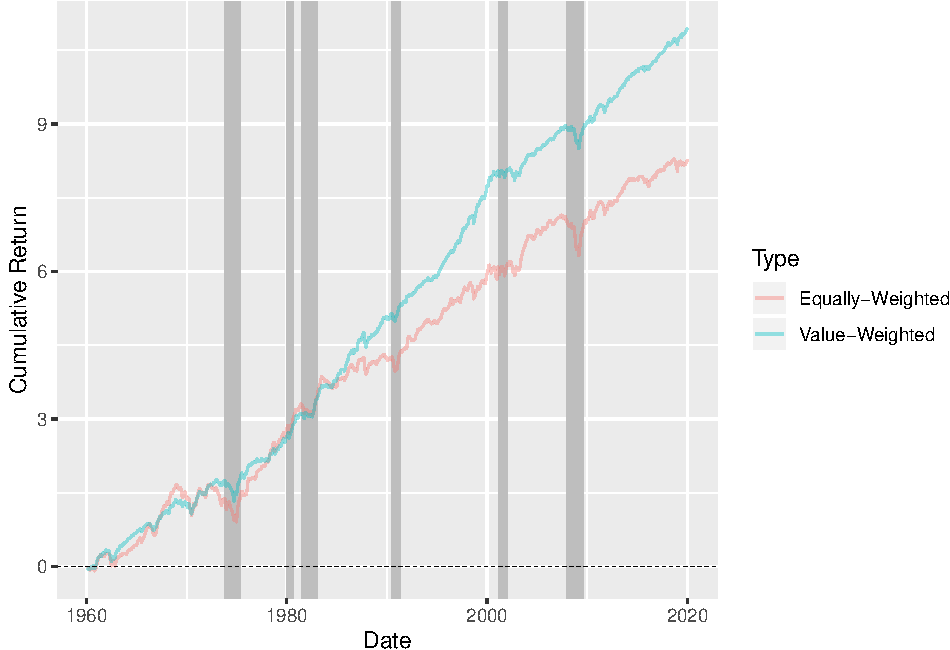
\includegraphics[width = 4in]{CRSP_COMP_files/figure-latex/unnamed-chunk-12-1}
\end{center}
\end{figure}

\end{Schunk}

We note that, overall, the equally-weighted portfolio under-performs the
value-weighted one. The equally-weighted portfolio attributes greater
weight to small-cap stocks. Contrary to \cite{fama1993common}, interestingly, we
observe that the value-weighted stocks outperform the small-cap stocks.
Nonetheless, the pattern became evident beginning in the late
80s. To take a closer look at the above, we group securities into size
portfolios. At each month, we group securities into 5 groups based on
the market cap cut-off.\footnote{\color{black}Note that in empirical asset pricing studies, when forming portfolios based on a single characteristic (i.e., single-sort), the common practice is to choose $G = 10$. On the other hand, for double-sorting it is common to choose $G = 5$. This, however, depends on data availability. In our case, we choose $G = 5$ for both brevity and consistency 
 (see, e.g., \cite{fama1993common}).} To perform the cut-off, we refer to the
\code{ntile} function from the \pkg{dplyr} library. In the
following analysis, we proceed with equal-weighting for the sake of
brevity.
\begin{Schunk}
\begin{Sinput}
library(dplyr)
cut.n <- 5
DT <- DT[,`:=` (Group_Size = ntile(MKTCAP,cut.n)), by = list(date)]
N_G <- DT[,.N, by = list(date,Group_Size) ]
N_G[,mean(N), by = list(Group_Size)]
\end{Sinput}
\begin{Soutput}
#>    Group_Size       V1
#> 1:          2 885.3694
#> 2:          1 885.7667
#> 3:          3 885.3875
#> 4:          4 885.3694
#> 5:          5 884.9500
\end{Soutput}
\end{Schunk}

We observe that, on average, each group contains 885 firms over the
sample period. In addition to the group size, we consider the next one
month return on each security. We use the \code{shift} function from
\pkg{data.table} and apply it to each security as follows:

\begin{Schunk}
\begin{Sinput}
DT <- DT[order(DT$CUSIP,DT$date),]
DT <- DT[,`:=` (RET_1 = shift(RET,-1)), by = list(CUSIP)]
\end{Sinput}
\end{Schunk}
Given the above, we report summary statistics on the size group level:
\begin{Schunk}
\begin{Sinput}
DT_size <- DT[,lapply(.SD,mean,na.rm = TRUE),by = list(Group_Size),
              .SDcols = c("RET","RET_1","PRC","SHROUT","MKTCAP","EXCHCD")]
DT_size <- DT_size[order(DT_size$Group_Size),]
DT_size$RET_1 <- DT_size$RET_1*12
DT_size$RET <- DT_size$RET*12
DT_size
\end{Sinput}
\begin{Soutput}
#>    Group_Size        RET     RET_1        PRC     SHROUT     MKTCAP   EXCHCD
#> 1:          1 -0.1047989 0.2177438   4.265575   7569.757   13946.99 2.704329
#> 2:          2  0.1463509 0.1069973   9.280118  11101.177   56211.45 2.592039
#> 3:          3  0.2047528 0.1200868  15.410881  15797.729  168506.54 2.396027
#> 4:          4  0.2313902 0.1266713  25.020412  26814.684  538252.87 2.039177
#> 5:          5  0.2132456 0.1225963 105.854839 167534.402 7505924.35 1.457429
\end{Soutput}
\end{Schunk} %$

Clearly, securities ranked in the 5th largest size group have a higher
market-cap, which is associated with  higher prices and shares
outstanding. Additionally, note that the large stocks are more likely to
be listed on NYSE (EXCHCD = 1), whereas the small-cap stocks are listed
on NASDAQ (EXCHCD = 3). In terms of returns, the results are sensitive
with respect to whether we consider an in-sample return or next month's return. In the in-sample, we observe that large-cap outperform small-cap. Nonetheless, the more relevant case in practice is the
out-of-sample return. In the latter case, we observe that small-cap
stocks outperform large-cap stocks. In annual terms, the small-cap stocks return 10\% higher mean return than large-cap stocks. Ignoring transaction cost and assuming that
investors rebalance their portfolios on a monthly basis, this evidence
is consistent with 
\cite{fama1993common}'s size premium. That is, investors expect
a higher return for investing in small-cap stocks.

\hypertarget{compustat}{%
\subsection{COMPUSTAT}\label{compustat}}

The above discussion relates to the CRSP data alone. In the following, we
focus on the COMPUSTAT data, which contains accounting-related
information for public firms. Similar to the
above, we focus on a subset of variables. For identification, we look into
the CUSIP and the CIK number. The latter is relevant to identify firms
via the SEC EDGAR system - for those interested in merging the data with
SEC filings and perform textual analysis. The \code{FYEARQ} and
\code{FQTR} are the fiscal year and quarter of the data point. For
accounting variables, we consider total assets (\code{atq}), net income
(\code{niq}), and common equity \code{ceqq}.

\begin{Schunk}
\begin{Sinput}
file.j <- "COMPUSTAT_1960_2020.csv"
select.var2 <- tolower(c("FYEARQ","FQTR","cusip","cik","sic","niq","atq","ceqq"))
DT2  <- unique(fread(file.j,select = select.var2))
\end{Sinput}
\end{Schunk}

\hypertarget{filters-and-cleaning-1}{%
\subsubsection{Filters and Cleaning}\label{filters-and-cleaning-1}}

To link between COMPUSTAT and CRSP, we need to make a small adjustment
for the CUSIP identifiers. In CRSP, the number of characters is 8,
whereas in COMPUSTAT, it is 9.

\begin{Schunk}
\begin{Sinput}
table(nchar(DT$CUSIP))
\end{Sinput}
\begin{Soutput}
#> 
#>       8 
#> 3187327
\end{Soutput}
\end{Schunk}

\begin{Schunk}
\begin{Sinput}
table(nchar(DT2$cusip))
\end{Sinput}
\begin{Soutput}
#> 
#>       0       9 
#>     130 1806228
\end{Soutput}
\end{Schunk}
Note that there a few cases in which the CUSIP is unavailable in
COMPUSTAT. The adjustments are described below:
\begin{Schunk}
\begin{Sinput}
DT2 <- DT2[!nchar(DT2$cusip) == 0,]
DT2$CUSIP <- substr(DT2$cusip,0,8)
DT2$cusip <- NULL
DT2 <- unique(DT2[DT2$CUSIP %in% DT$CUSIP,])
\end{Sinput}
\end{Schunk}

In order to merge with the CRSP data, which corresponds to calendar
dates, we adjust the fiscal dates in COMPUSTAST. It is common to use 6
months lags to allow the financial disclosures to become publicly
available. To do so, we perform the following adjustments:

\begin{Schunk}
\begin{Sinput}
DT2$date <- ymd(DT2$fyearq*10000 + DT2$fqtr*3*100 + 1)
DT2$date <- DT2$date + months(6)
DT2$date <- ceiling_date(DT2$date,"q") - 1
DT2 <- DT2[month(DT2$date) == 6,]
DT2$fyearq <- DT2$fqtr <- NULL
\end{Sinput}
\end{Schunk}
Additionally, we keep the annual data rather than the quarterly one and consider portfolio formation on an annual basis.\footnote{Clearly, it all depends on the purpose of the investigation.}
In
particular, we keep the June data for the portfolio formation
process.

Same as before, let us check for duplicates:
\begin{Schunk}
\begin{Sinput}
DT2 <- unique(DT2)
DT2[ , `:=`( duplicate_N = .N   ) , by= list(CUSIP,date)]
table(DT2$duplicate_N)
\end{Sinput}
\begin{Soutput}
#> 
#>      1 
#> 247903
\end{Soutput}
\begin{Sinput}
DT2$duplicate_N <- NULL
\end{Sinput}
\end{Schunk}
The COMPUSTAT dataset have unique CUSIP-date observations.

\hypertarget{summary-statistics}{%
\subsubsection{Summary Statistics}\label{summary-statistics}}

Given the final COMPUSTAT data, we consider a few summary statistics for
each industry, which is defined using the 4th digit of the SIC code.

\begin{Schunk}
\begin{Sinput}
DT2 <- na.omit(DT2)
DT2$ROA <- DT2$niq/DT2$atq
DT2$ROE <- DT2$niq/DT2$ceqq
DT2$BL <- DT2$atq/DT2$ceqq
DT2$Industry <- floor(DT2$sic/1000)

DT2_sum <- DT2[,lapply(.SD,median,na.rm = TRUE), by = list(Industry),
               .SDcols = c("atq","ROA","ROE","BL")]
DT2_sum <- DT2_sum[order(DT2_sum$Industry),]
DT2_sum
\end{Sinput}
\begin{Soutput}
#>     Industry      atq          ROA          ROE       BL
#>  1:        0  97.9455 -0.005973224 -0.007163557 2.005072
#>  2:        1 152.8265  0.003908058  0.015030814 2.031069
#>  3:        2 112.5905  0.006157001  0.023091766 1.761200
#>  4:        3  85.0685  0.010216054  0.024022369 1.736357
#>  5:        4 540.3000  0.006908974  0.024877318 2.914309
#>  6:        5 148.0990  0.011941449  0.030180501 2.155898
#>  7:        6 893.6370  0.002491525  0.026317412 8.965721
#>  8:        7  88.5455  0.004830920  0.018396345 1.736342
#>  9:        8  73.5180  0.006937877  0.020926220 1.904278
#> 10:        9  37.3550 -0.003438435  0.006888589 1.562943
\end{Soutput}
\end{Schunk}
We observe that financial firms are associated with the highest book leverage,
given the business nature of financial institutions. Also, we note that
the financial industry is associated with the largest total assets. This
is not surprising given the concentration of the financial industry over
time, in which a few entities hold the majority of assets. To relate to
the last point, consider the total assets of the top 10\% firms with
respect to the total assets in the industry as a whole.

\begin{Schunk}
\begin{Sinput}
DT2_Fin <- DT2[DT2$Industry == 6,]
DT2_Fin <- DT2_Fin[,`:=` (Group_Size = ntile(atq,10)), by = list(date)]
DT2_Fin <- DT2_Fin[,`:=` (Total_Assets = sum(atq)), by = list(date)]
DT2_Fin <- DT2_Fin[,lapply(.SD, function(x) sum(x/Total_Assets)), 
                   by = list(date,Group_Size), .SDcols = "atq"]
DT2_Fin_Top <- DT2_Fin[DT2_Fin$Group_Size == 10,]
DT2_Fin_Top <- DT2_Fin_Top[order(DT2_Fin_Top$date),]
plot(atq~date,data = DT2_Fin_Top,type = "l",
     main = "Proportion of Assets held by Top 10% in Financial Industry",
     ylab = "", xlab = "Date")
grid(10)
\end{Sinput}
%$
\end{Schunk}
\begin{figure}
\caption{This figure below demonstrates the concentration in the financial industry. It illustrates the book value of assets held by the top 10\% banks relative to the total assets held by the financial industry.}
\label{fig:banks}
\begin{center}
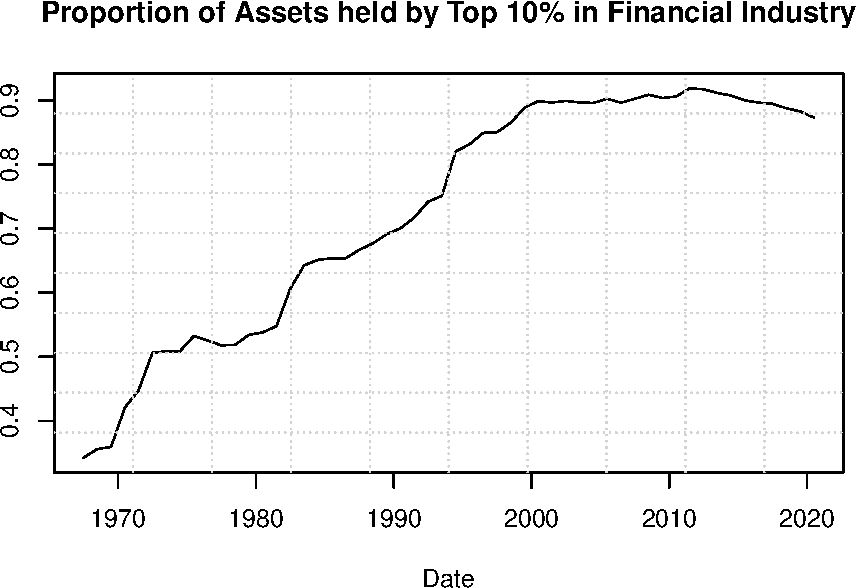
\includegraphics[width = 4in]{CRSP_COMP_files/figure-latex/unnamed-chunk-23-1} 
\end{center}
\end{figure}

According to Figure \ref{fig:banks}, we  discern that the top 10\% increased their share of total assets from
34\% in the late 60s up to 90\% more recently.

\hypertarget{crsp-compustat}{%
\subsection{CRSP-COMPUSTAT}\label{crsp-compustat}}
Note that the COMPUSTAT dataset is annual, while the CRSP is monthly.
If we seek to form portfolios based on book-to-market (BM) ratio, such as
the case for Fama-French, we need to create an  annual BM variable in the
COMPUSTAT dataset. Before we merge the data altogether, let us add the
market value of equity (ME) to the COMPUSTAT dataset. Additionally, we
add the stock prices which would be useful for small-cap stocks
from the portfolio formation later on.

\begin{Schunk}
\begin{Sinput}
BM <- DT[,c("date","CUSIP","MKTCAP","PRC")]
DT2 <- merge(DT2,BM, by = c("CUSIP","date"), all = F)
DT2$BM_ratio <- DT2$ceqq/(DT2$MKTCAP/1000)
DT2$ME <- DT2$MKTCAP
DT2$PRC_LAST <- DT2$PRC
DT2$MKTCAP <-  DT2$PRC <- NULL
DT2 <- DT2[order(DT2$CUSIP,DT2$date),]
DT2[,`:=` (N_years = 1:.N), by = list(CUSIP)]
rm(BM); gc()
\end{Sinput}
\begin{Soutput}
#>            used  (Mb) gc trigger   (Mb)  max used   (Mb)
#> Ncells  1024743  54.8    2730065  145.9   2730065  145.9
#> Vcells 63598437 485.3  149041274 1137.1 148737297 1134.8
\end{Soutput}
\end{Schunk} %$
The above commands link the COMPUSTAT and the CRSP datasets to
determine the market equity of the firms and, hence, the book-to-market
ratio. Also, we denote the stock price as \code{PRC\_LAST} to refer to
the recent stock price in the annual data.

Before we finally merge the data altogether, we need to do one small
trick with the CRSP data. The ultimate goal of this illustration to
attribute the next 12 months' returns with respect to the BM ratio from
the previous June. To do so, consider the following:
\begin{Schunk}
\begin{Sinput}
prev_june_f <- function(x) floor_date(floor_date(x,"m") + months(6),"y") - months(6) - 1
DT$date_june <- prev_june_f(DT$date)
DT2$date_june <- DT2$date
DT2$date <- NULL
\end{Sinput}
\end{Schunk} %$
While the \code{prev\_june\_f} seems obscure, one should break the
function into different components in order to understand how it works.
Consider the special case where we have:
\begin{Schunk}
\begin{Sinput}
x <- DT$date[1:13]
x
\end{Sinput}
\begin{Soutput}
#>  [1] "1970-12-31" "1971-01-31" "1971-02-28" "1971-03-31" "1971-04-30"
#>  [6] "1971-05-31" "1971-06-30" "1971-07-31" "1971-08-31" "1971-09-30"
#> [11] "1971-10-31" "1971-11-30" "1971-12-31"
\end{Soutput}
\end{Schunk} %$
The first command of the function shifts the dates six months ahead:
\begin{Schunk}
\begin{Sinput}
floor_date(x,"m") + months(6)
\end{Sinput}
\begin{Soutput}
#>  [1] "1971-06-01" "1971-07-01" "1971-08-01" "1971-09-01" "1971-10-01"
#>  [6] "1971-11-01" "1971-12-01" "1972-01-01" "1972-02-01" "1972-03-01"
#> [11] "1972-04-01" "1972-05-01" "1972-06-01"
\end{Soutput}
\end{Schunk}
The second step identifies the floor of each date on the annual level:
\begin{Schunk}
\begin{Sinput}
floor_date(floor_date(x,"m") + months(6),"y")
\end{Sinput}
\begin{Soutput}
#>  [1] "1971-01-01" "1971-01-01" "1971-01-01" "1971-01-01" "1971-01-01"
#>  [6] "1971-01-01" "1971-01-01" "1972-01-01" "1972-01-01" "1972-01-01"
#> [11] "1972-01-01" "1972-01-01" "1972-01-01"
\end{Soutput}
\end{Schunk}
The final step subtracts 6 months to identify the June of the previous
year. The minus one is added to retrieve June 30th rather than July
1st, such that:
\begin{Schunk}
\begin{Sinput}
floor_date(floor_date(x,"m") + months(6),"y") - months(6) - 1
\end{Sinput}
\begin{Soutput}
#>  [1] "1970-06-30" "1970-06-30" "1970-06-30" "1970-06-30" "1970-06-30"
#>  [6] "1970-06-30" "1970-06-30" "1971-06-30" "1971-06-30" "1971-06-30"
#> [11] "1971-06-30" "1971-06-30" "1971-06-30"
\end{Soutput}
\end{Schunk}


\begin{figure}[!ht]
\begin{center}
\caption{ \color{black} The figure below illustrates a flow chart of the data merging process. It demonstrates the steps taken altogether to come up with the final CRSP-COMPUSTAT merged data set. }
\label{figure:flowchart}
\fbox{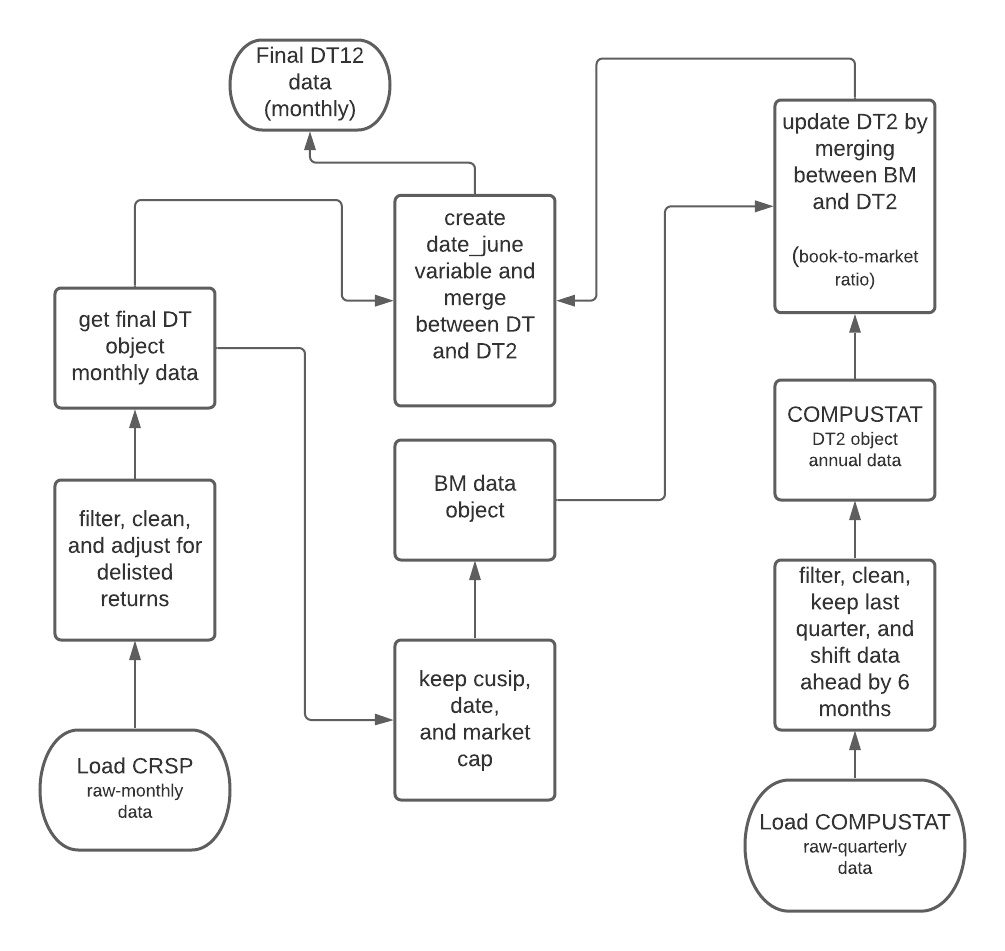
\includegraphics[width = 4in]{flow_chart}} 
\end{center}
\end{figure}

Looking at returns between Dec 1970 and Mar 1971, the function traces
these observations back to June 1970 for the first 7 returns. When the
next June data shows up, the \code{date\_june} variable adjusts
accordingly. Finally, the merged dataset is given by:

\begin{Schunk}
\begin{Sinput}
DT12 <- merge(DT,DT2,by = c("CUSIP","date_june")) 
\end{Sinput}
\end{Schunk}

{\color{black}
\noindent \textbf{Note}: The above steps provide details on how to merge between the two data sets. In Figure \ref{figure:flowchart}, we provide a flow chart summarizing the steps/processes undertaken to develop the final merged data set \code{DT12}.
}


\hypertarget{forming-size-and-bm-portfolios}{
\section{Forming Size and BM
Portfolios}
\label{forming-size-and-bm-portfolios}
}

The \code{DT12} object contains the final CRSP-COMPUSTAT data. The
merging is conducted to allow for portfolio formation at the end of June
each year, as mentioned above. Such a setting allows a convenient way to form
portfolios without relying on loops. Nonetheless, it
would also impose that portfolio managers balance their portfolios on a
monthly basis according to the market cap from the previous June.

Given the merged dataset, we form groups at the end of June-year based
on market equity (size) and book-to-market ratio (value):

\begin{Schunk}
\begin{Sinput}
DT12 <- DT12[,`:=` (Group_ME = ntile(ME,5)), by = list(date_june)]
DT12 <- DT12[,`:=` (Group_BM = ntile(BM_ratio,5)), by = list(date_june,Group_ME)]
\end{Sinput}
\end{Schunk}
The above two commands perform dependent portfolio sorting, in which 
firms are first sorted based on size and then on BM ratio. We
consider value-weighting to compute the future returns on each
size-value portfolio. This results in 25 value-weighted portfolios.

\begin{Schunk}
\begin{Sinput}
PORT_RET <- DT12[,list(VW_RET = sum(RET*ME/sum(ME))  ),
                 by = list(date,Group_ME,Group_BM)]
PORT_RET <- PORT_RET[order(PORT_RET$date,PORT_RET$Group_BM,PORT_RET$Group_ME),]
PORT_RET$VW_RET <- as.numeric(PORT_RET$VW_RET)*100

ret_matrix <- PORT_RET[,lapply(.SD,mean,na.rm = TRUE),
                       by = list(Group_ME,Group_BM), .SDcols = "VW_RET"]
ret_matrix <- ret_matrix[order(ret_matrix$Group_BM,ret_matrix$Group_ME),]
ret_matrix <- matrix(as.numeric(ret_matrix$VW_RET),5)
rownames(ret_matrix) <- 1:5
colnames(ret_matrix) <- paste("BM",1:5,sep = "_")
rownames(ret_matrix)[1] <- "Small"
rownames(ret_matrix)[5] <- "Big"
colnames(ret_matrix)[1] <- "Low"
colnames(ret_matrix)[5] <- "High"
round(data.frame(ret_matrix*12),2)
\end{Sinput}
\begin{Soutput}
#>         Low  BM_2  BM_3  BM_4  High
#> Small 12.93 14.73 18.05 20.14 23.40
#> 2      8.45 12.55 14.37 16.72 16.17
#> 3      8.04 11.79 14.30 14.24 15.99
#> 4      9.89 11.53 11.92 14.47 14.77
#> Big    9.84 11.70 10.41 13.13 12.78
\end{Soutput}
\end{Schunk}

For each column above, we observe the stock returns (raw) decrease, on
average, with size. This is commonly known as the size effect. At the
same time, we observe that within each size group, the mean return
increases with the BM ratio. The latter denotes what is known as the value
effect. In other words, investors expect higher returns from small
enterprises and undervalued stocks (trading below book value).
Nonetheless, recent discussions debate whether this is the case. For
further information on this, see this
\href{https://www.bloomberg.com/news/articles/2020-02-06/quant-pioneers-of-value-investing-are-trying-to-see-if-it-s-dead}{article}.

\hypertarget{risk-adjusted-returns-using-fama-french-risk-factors}{%
\subsection{Risk-Adjusted Returns using Fama-French's Risk
Factors}\label{risk-adjusted-returns-using-fama-french-risk-factors}}

The above portfolio results compute the raw returns. In order to price
these portfolios, we decompose the returns into (1) systematic components
(risk-premiums) and (2) non-systematic. The latter denotes the risk-adjusted
returns. Additionally, we consider the excess return on each portfolio,
i.e., the portfolio return minus the 1-month Treasury yield.

The Fama-French's risk factors are obtained easily using the Kenneth French
public \href{http://mba.tuck.dartmouth.edu/pages/faculty/ken.french/}{library} according to the commands below. Note that we focus on the
three factors: market, size, and value:

\begin{Schunk}
\begin{Sinput}
FF_file <- 
  "https://mba.tuck.dartmouth.edu/pages/faculty/ken.french/ftp/F-F_Research_Data_Factors_CSV.zip"
temp <- tempfile()
download.file(FF_file,temp)
unz_files <- unzip(temp)
ds <- read.csv(unz_files,skip = 3)
flag_obs <- grep("Annual",ds[,1],ignore.case = TRUE)
ds <- ds[1:(flag_obs-1),]
names(ds)[1] <- "date"
ds <- data.frame(apply(ds, 2, as.numeric))
ds$date <- ceiling_date(ymd(ds$date*100+ 01),"m")-1
tail(ds)
\end{Sinput}
\begin{Soutput}
#>            date Mkt.RF   SMB    HML   RF
#> 1123 2020-01-31  -0.11 -3.11  -6.27 0.13
#> 1124 2020-02-29  -8.13  0.96  -4.01 0.12
#> 1125 2020-03-31 -13.39 -5.16 -14.12 0.12
#> 1126 2020-04-30  13.65  2.78  -1.27 0.00
#> 1127 2020-05-31   5.58  2.47  -4.95 0.01
#> 1128 2020-06-30   2.45  2.56  -2.03 0.01
\end{Soutput}
\end{Schunk}

We merge the risk factors data with the portfolios
time series  and regress the excess returns of each of the 25 portfolios on the three
factors. To do so, we leverage some functional programming
using the \code{lapply} base function along with the \code{dlply}
function from the \pkg{plyr} library as follows:
\begin{Schunk}
\begin{Sinput}
PORT_RET_RA <- merge(PORT_RET,ds)
PORT_RET_RA$RAR <- PORT_RET_RA$VW_RET - PORT_RET_RA$RF

lm_list <- dlply(PORT_RET_RA,c("Group_ME","Group_BM"),
                 function(x)  lm( RAR ~ Mkt.RF +  SMB +   HML, data = x   )    )  
rar_matrix <- lapply(lm_list, coef)
rar_matrix <- sapply(rar_matrix,function(x) x[[1]])
rar_matrix <- matrix(rar_matrix,5,5,byrow = TRUE)

rownames(rar_matrix) <- 1:5
colnames(rar_matrix) <- paste("BM",1:5,sep = "_")
rownames(rar_matrix)[1] <- "Small"
rownames(rar_matrix)[5] <- "Big"
colnames(rar_matrix)[1] <- "Low"
colnames(rar_matrix)[5] <- "High"

rar_matrix <- round(data.frame(rar_matrix*12),2)
rar_matrix
\end{Sinput}
\begin{Soutput}
#>         Low  BM_2  BM_3  BM_4  High
#> Small -1.08  2.03  5.55  6.49  8.90
#> 2     -5.77 -0.33  0.78  2.47  1.01
#> 3     -6.51 -1.66  0.96 -0.15 -0.18
#> 4     -2.90 -1.41 -0.90  0.08 -0.10
#> Big    0.35  1.47 -0.47  0.32 -1.29
\end{Soutput}
\end{Schunk} %$

Note that after controlling for the three risk factors, the high-small
portfolio still yields an annual return of 9\%. A potential argument may
be that such alpha is attributed to other risk factors that the
three-factor model does not fully  price. More recently, Fama-French suggest
five factors model to better representation of systematic components
\citep{fama2015five}.

\hypertarget{rendering-results}{%
\section{Rendering Results}\label{rendering-results}}

The above results are subjected to certain filtering, the time period,
and the number of months each stock should include in the data. One
major challenge is whether the securities in the analysis are tradable.
For instance, it is common to consider stocks with a price larger than
\$5. The major issue with doing so is that such a filter could cause a
forward-looking bias. By the time the decision maker allocates his/her
portfolio, he/she cannot ascertain whether the stocks would be above or
less than \$5 in the future - this is less of an issue for large-cap stocks.
Hence, to keep stocks that satisfy a minimum price level, it
should be done on a recurring basis. Specifically, rather than dropping all
observations in which the price is less than \$5, one should consider only
the stocks that were qualified by the time of the portfolio formation.
The same issue applies to the window length for which the data is
available  and other filters one may be interested in controlling for.




The following is a generalized portfolio formation function that takes
four arguments. The first two correspond to the minimum price and number of years that the stock should have to be considered investable in June each year. The other two arguments set the time period during which the researcher is interested in computed the mean returns. The function returns a list containing the raw and risk-adjusted returns of the 25 portfolios along with the average number of stocks within each
portfolio.
\begin{Schunk}
\begin{Sinput}
FF3_anomaly <- function(min_price,year_keep = 1,year1 = 1965,year2 =  2019) {
  DT12_sub <- DT12
  keep_cusip_date <- unique(DT12_sub[,list(CUSIP,date_june,N_years,PRC_LAST)])
  keep_cusip_date <- keep_cusip_date[keep_cusip_date$N_years >= year_keep,]
  keep_cusip_date <- keep_cusip_date[keep_cusip_date$PRC_LAST >= min_price ,]
  
  keep_cusip_date <- unique(keep_cusip_date[,list(CUSIP,date_june)])
  DT12_sub <- merge(DT12_sub,keep_cusip_date)
  
  DT12_sub <- DT12_sub[,`:=` (Group_ME = ntile(ME,5)), by = list(date_june)]
  DT12_sub <- DT12_sub[,`:=` (Group_BM = ntile(BM_ratio,5)), by = list(date_june,Group_ME)]
  N_G <- DT12_sub[,.N, by = list(date,Group_ME,Group_BM) ]
  N_G <- (N_G[,mean(N), by = list(Group_ME,Group_BM) ])
  N_G <- N_G[order(N_G$Group_ME,N_G$Group_BM),] 
  N_G <- matrix(N_G$V1,5,5,byrow = TRUE)
  rownames(N_G) <- 1:5
  colnames(N_G) <- paste("BM",1:5,sep = "_")
  rownames(N_G)[1] <- "Small"
  rownames(N_G)[5] <- "Big"
  colnames(N_G)[1] <- "Low"
  colnames(N_G)[5] <- "High"
  N_G <- round((N_G))
  
  PORT_RET <- DT12_sub[,list(VW_RET = sum(RET*ME/sum(ME))  ),
                       by = list(date,Group_ME,Group_BM)]
  PORT_RET <- PORT_RET[order(PORT_RET$date,PORT_RET$Group_BM,PORT_RET$Group_ME),]
  PORT_RET$VW_RET <- as.numeric(PORT_RET$VW_RET)*100
  
  PORT_RET_RA <- merge(PORT_RET,ds)
  PORT_RET_RA$RAR <- PORT_RET_RA$VW_RET - PORT_RET_RA$RF
  PORT_RET_RA_sub <- PORT_RET_RA
  PORT_RET_RA_sub <- PORT_RET_RA_sub[year(PORT_RET_RA_sub$date) >= year1,] 
  PORT_RET_RA_sub <- PORT_RET_RA_sub[year(PORT_RET_RA_sub$date) <= year2 ,] 
  
  ret_matrix <- PORT_RET_RA_sub[,lapply(.SD,mean,na.rm = TRUE),
                                by = list(Group_ME,Group_BM), .SDcols = "VW_RET"]
  ret_matrix <- ret_matrix[order(ret_matrix$Group_BM,ret_matrix$Group_ME),]
  ret_matrix <- matrix(as.numeric(ret_matrix$VW_RET),5)
  rownames(ret_matrix) <- 1:5
  colnames(ret_matrix) <- paste("BM",1:5,sep = "_")
  rownames(ret_matrix)[1] <- "Small"
  rownames(ret_matrix)[5] <- "Big"
  colnames(ret_matrix)[1] <- "Low"
  colnames(ret_matrix)[5] <- "High"
  ret_matrix <- round(data.frame(ret_matrix*12),2)
  
  
  lm_list <- dlply(PORT_RET_RA_sub,c("Group_ME","Group_BM"), 
                   function(x)  lm( RAR ~ Mkt.RF +  SMB +   HML, data = x   )    )  
  rar_matrix <- lapply(lm_list, coef)
  rar_matrix <- sapply(rar_matrix,function(x) x[[1]])
  rar_matrix <- matrix(rar_matrix,5,5,byrow = TRUE)
  rownames(rar_matrix) <- 1:5
  colnames(rar_matrix) <- paste("BM",1:5,sep = "_")
  rownames(rar_matrix)[1] <- "Small"
  rownames(rar_matrix)[5] <- "Big"
  colnames(rar_matrix)[1] <- "Low"
  colnames(rar_matrix)[5] <- "High"
  rar_matrix <- round(data.frame(rar_matrix*12),2)
  
  
  list(N_G,ret_matrix,rar_matrix)
  
}
\end{Sinput}
\end{Schunk}

\hypertarget{control-for-minimum-price}{%
\subsubsection{Control for Minimum
Price}\label{control-for-minimum-price}}

Given the above function, we test the sensitivity of the size/value
premiums by including stocks with pre-specified minimum price. In
particular, we run this for a sequence of prices ranging between 0 and
\$50. With the \pkg{parallel} library, we can easily perform parallel
computing on four cores. It takes a few seconds to run the following commands\footnote{Note that the \code{mclapply} can be easily leveraged on Linux machines.}:
\begin{Schunk}
\begin{Sinput}
p_seq <- 0:50
list_port_price <- mclapply(p_seq, function(p) FF3_anomaly(p),mc.cores = 4)
\end{Sinput}
\end{Schunk}

Given the list \code{list\_port\_price}, we extract the result of
interest. In this case, we focus on the raw returns. For instance, the
first item of this list corresponds to the same results from Section \ref{forming-size-and-bm-portfolios}.
\begin{Schunk}
\begin{Sinput}
list_port_price[[1]][[2]]
\end{Sinput}
\begin{Soutput}
#>         Low  BM_2  BM_3  BM_4  High
#> Small 12.93 14.73 18.05 20.14 23.40
#> 2      8.45 12.55 14.37 16.72 16.17
#> 3      8.04 11.79 14.30 14.24 15.99
#> 4      9.89 11.53 11.92 14.47 14.77
#> Big    9.84 11.70 10.41 13.13 12.78
\end{Soutput}
\end{Schunk}
On the other hand, if we consider \$5 minimum price, we see that the
results are tentative depending on the level of entry:
\begin{Schunk}
\begin{Sinput}
list_port_price[[6]][[2]]
\end{Sinput}
\begin{Soutput}
#>         Low  BM_2  BM_3  BM_4  High
#> Small  8.86 12.19 14.64 15.31 17.86
#> 2     10.35 11.94 13.51 16.18 15.08
#> 3      8.54 12.39 13.52 14.41 15.07
#> 4     10.16 11.09 11.95 14.20 15.17
#> Big    9.79 11.66 10.62 12.95 12.42
\end{Soutput}
\end{Schunk}

To capture this for each matrix of raw returns, we compute the
high-minus-low (HML), i.e., column 5 minus column 1 for each size
level. This results in 5 HML premiums for each size level. We summarize
the results in Figure \ref{fig:value_effect}.

\begin{Schunk}
\begin{Sinput}
RAR_list <- lapply(list_port_price,function(x) x[[2]])
RAR_list_Value <- t(sapply(RAR_list, function(x) x[,5] - x[,1]  ))
colnames(RAR_list_Value) <- rownames(RAR_list[[1]])
RAR_list_Size <- t(sapply(RAR_list, function(x) x[1,] - x[5,]  ))

ds.plot <- lapply(1:5, function(i) data.frame(HML =  RAR_list_Value[,i],
                                              Min_Price = p_seq, Size = i))
ds.plot <- Reduce(rbind,ds.plot)
ds.plot <- ds.plot[order(ds.plot$Size,ds.plot$Min_Price),]
ds.plot <- ds.plot[ds.plot$Size %in% c(1,3,5),]
ds.plot$Size <- as.factor(ds.plot$Size)
p <- ggplot(ds.plot,aes(x = Min_Price, y = HML, colour = Size, shape = Size))
p <- p + geom_point() + geom_line()
p <- p + geom_abline(intercept = 0, slope = 0, color="black",  linetype="dashed")
p
\end{Sinput}  

\begin{figure}
\caption{This figure summarizes the results of the double-sorting portfolio based on the book-to-market (BM) ratio and size. Stocks are first sorted into five quintiles with respect to the BM ratio. Then, within each BM quintile, stocks are sorted based on size. The double-sorting results in 25 value-weighted portfolios. The $y$-axis corresponds to the value premium, which is the difference between the top and the bottom BM quintiles within a given size group. The $x$-axis controls for the stock's minimum price to be included within each one of the 25 sorted portfolios. The red, green, and blue lines correspond to the size groups of small-cap (1), medium-cap (2), and large-cap (5), respectively. Overall, the plot demonstrates the sensitivity of the value premium as a function of the minimum price. 
}
\label{fig:value_effect}
    \begin{center}
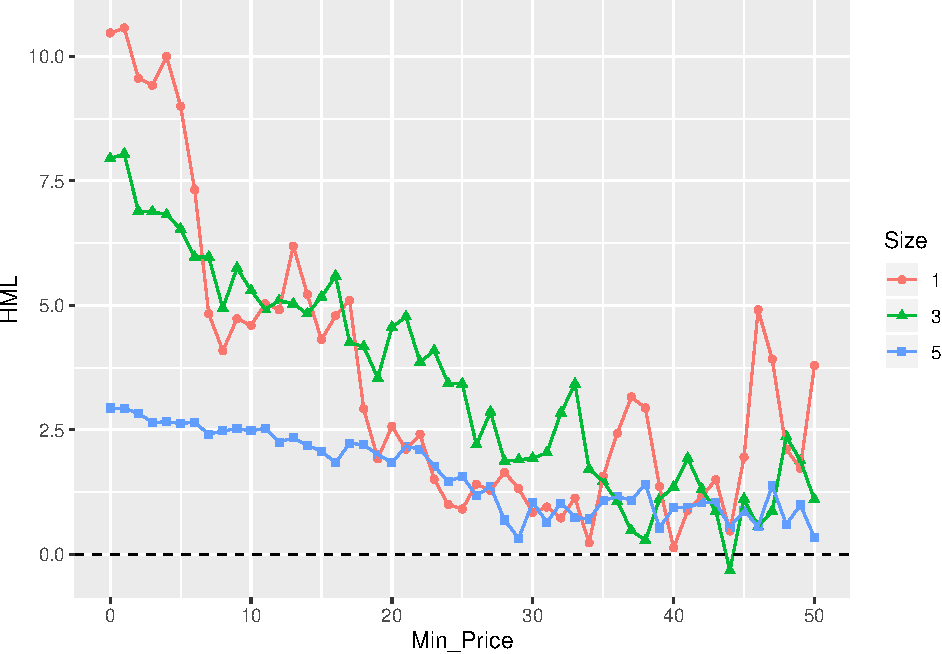
\includegraphics[width = 3.5in]{CRSP_COMP_files/figure-latex/unnamed-chunk-40-1}
 \end{center}
\end{figure}
\end{Schunk}
%$



We observe that the HML is more evident for small-cap stocks. However,
at the same time, we note that the premium declines as we increase the minimum price entry. One argument is the following. As we increase the minimum price, the size effect is mitigated and, hence, the value premium. On the other hand, this could also be attributed to whether
investors can utilize such alphas for small-cap that tend to be less
liquid.

We repeat the same plot for the size premium. In particular, we compute the small-minus-big (SMB), i.e., row 1 minus row 5 for each BM level. This results in 5 SMB premiums for each BM group. Similar to Figure \ref{fig:value_effect}, Figure \ref{fig:size_effect} demonstrates the sensitivity of the results with respect to the minimum price:
\begin{Schunk}
\begin{Sinput}
ds.plot <- lapply(1:5, function(i) data.frame(SMB =  unlist(RAR_list_Size[,i]),
                                              Min_Price = p_seq, BM = i))
ds.plot <- Reduce(rbind,ds.plot)
ds.plot <- ds.plot[order(ds.plot$BM,ds.plot$Min_Price),]
ds.plot <- ds.plot[ds.plot$BM %in% c(1,3,5),]
ds.plot$BM <- as.factor(ds.plot$BM)
p <- ggplot(ds.plot,aes(x = Min_Price, y = SMB, colour = BM, shape = BM))
p <- p + geom_point() + geom_line()
p <- p + geom_abline(intercept = 0, slope = 0, color="black",  linetype="dashed")
p
\end{Sinput}
%$
\end{Schunk}

\begin{figure}
\caption{This figure summarizes the results of the double-sorting portfolio based on the book-to-market (BM) ratio and size. Stocks are first sorted into five quintiles with respect to the BM ratio. Then, within each BM quintile, stocks are sorted based on size. The double-sorting results in 25 value-weighted portfolios. The $y$-axis corresponds to the size premium, which is the difference between the top and the bottom size quintiles withing a given BM group. The $x$-axis controls for the stock's minimum price to be included within each one of the 25 sorted portfolios. The red, green, and blue lines correspond to different BM groups of low (1), medium (2), and high (5), respectively. Overall, the plot demonstrates the sensitivity of the size premium as a function of the minimum price. 
}
\label{fig:size_effect}
\begin{center}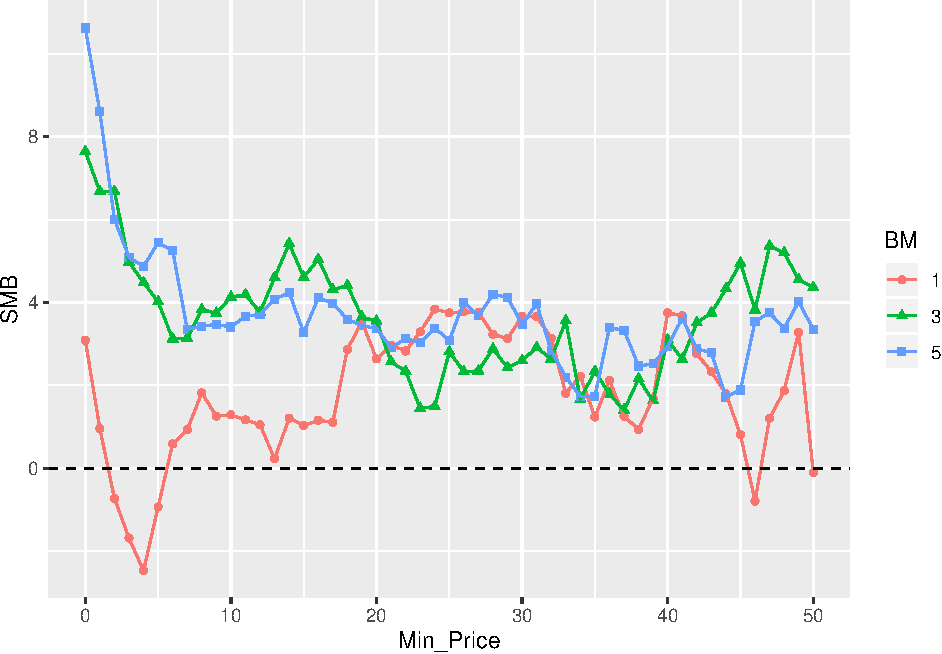
\includegraphics[width = 3.5in]{CRSP_COMP_files/figure-latex/unnamed-chunk-41-1} \end{center}
\end{figure}

Consistent with the case for the HML premium, the SMB premium seems to shrink as we increase the minimum price entry. While different forces could be attributed to this, it is of great relevance for researchers/investors to understand the mechanisms behind which. Interested readers may find the work by \citet{li2014limits} very relevant concerning the impact of liquidity and limits of arbitrage when it comes to the inclusion/exclusion of small-cap stocks.



\color{black}
\section{Additional Results}
We conduct one additional test related to the capital asset pricing model (CAPM) by \cite{sharpe1964capital} and \cite{lintner1965valuation}. The following analysis depends only on the CRSP database rather than the merged CRSP-COMPUSTAT data. Hence, the code is executed based on the \code{DT} data object only. 

The CAPM postulates a positive linear relationship between the market beta (systematic risk) and the asset's mean return. 
Empirically, a large body of research shows that the relationship is flatter than the one predicted by the model \citep{jensen1972capital} or even negative \citep{frazzini2014betting}.  Consistent with the literature \citep{bali2016empirical}, we sort stocks into 10 portfolios based on their monthly beta. 
In particular, we use $M$ months to estimate the market beta on a rolling window using the    \CRANpkg{rollRegres} \citep{rollRegress} library. We set $M$ to be either 36, 60, or 120 months. For each sample size $M$, we estimate the market beta on a rolling basis. At the end of month $t$, we sort stocks into 10 groups based on their market beta and compute the value-weighted return over the next month at $t+1$. For the next month, we repeat the same procedure until the last month of our data sample. 



\begin{Schunk}
\begin{Sinput}

BETA <- DT[,c("date","CUSIP","RET")]
BETA <- merge(BETA,ds[,c("date","Mkt.RF","RF")], by = "date")
BETA$E_RET <- (BETA$RET - BETA$RF/100)*100
BETA$RF <- NULL
# keep stocks with at least M months
BETA[, count := (.N), by = CUSIP]
BETA <- BETA[order(BETA$CUSIP,BETA$date),]
BETA <- BETA[BETA$count   > est_window,]

BETA <- BETA %>%
  group_by(CUSIP) %>%
  do(.,mutate(.,Beta = roll_regres(E_RET ~ Mkt.RF,data = .,est_window)$coef[,2]))

BETA <- data.table(BETA)
BETA <- na.omit(BETA[,list(date,CUSIP,Beta)])

DT_capm <- merge(DT,BETA, by = c("CUSIP","date"), all = F)
DT_capm <- DT_capm[order(DT_capm$CUSIP,DT_capm$date),]
DT_capm <- DT_capm[,`:=` (Group_Beta = ntile(Beta,10)), by = list(date)]

\end{Sinput}
\end{Schunk}






Note that we execute the \code{roll\_regres} command using the \code{do} command in the tidy environment. This approach is the fastest solution to execute a rolling regression for panel data to the best of our knowledge. For instance, when $M = 120$, the \code{DT\_capm} data object contains 1,287,611 observations with 9,149 unique securities. The execution takes about 10 seconds.  Given the data object \code{DT\_capm}, we compute the next month's portfolio value-weighted return as follows:

\begin{Schunk}
\begin{Sinput}

PORT_RET <- DT_capm[,list(VW_RET = 12*100*sum(RET_1*MKTCAP/sum(MKTCAP),na.rm = T),
                          VW_BETA = sum(Beta*MKTCAP/sum(MKTCAP),na.rm = T)),
                    by = list(date,Group_Beta)]
PORT_RET <- PORT_RET[order(PORT_RET$Group_Beta,PORT_RET$date),]
\end{Sinput}
\end{Schunk}



Finally, we summarize the results using \pkg{ggplot2} in Figure \ref{fig:sim}. Note that the dashed line denotes the relationship implied by the CAPM. Figure \ref{fig:sim} is consistent with Figure 2 from \cite{fama2004capital}, where the slope (intercept) denotes the average annual market excess (risk-free) return. We compute the slope and intercept of the CAPM line based on the sub-sample of the Fama-French data set \code{ds} that corresponds to the same dates of the portfolio returns.



\begin{Schunk}
\begin{Sinput}
CAPM_result <- PORT_RET[,lapply(.SD,mean,na.rm = T),
                        by = list(Group_Beta), 
                        .SDcols = c("EW_RET","VW_RET","EW_BETA","VW_BETA")]
CAPM_result <- CAPM_result[order(CAPM_result$Group_Beta),]
CAPM_result

ds_sub <- ds[ds$date %in% PORT_RET$date,]

p2 <- ggplot(CAPM_result, aes(VW_BETA, VW_RET)) +
  geom_point()
p2 <- p2 + geom_smooth(method = "lm")
p2 <- p2 +ylim(c(5,15)) + xlim(c(0,2.5))
p2 <- p2 + geom_abline(intercept = mean(ds_sub$RF)*12, 
                       slope = mean(ds_sub$Mkt.RF)*12, 
                       color="red", linetype="dotted", size=1)


\end{Sinput}
\end{Schunk}






\begin{figure}[!ht] 
 \caption{\color{black} \textbf{Capital Asset Pricing Model} \\ The dots below report the average annualized monthly return  ($y$-axis) versus market beta   ($x$-axis) for the value-weighted portfolios. The solid line is smoothed using linear regression. The dashed line corresponds to the one predicted by the CAPM over the same sample period, where the slope (intercept) denotes the average annual market excess (risk-free) return. Each panel corresponds to a different estimation window needed to estimate the market beta and form beta portfolios on a rolling basis.}
\label{fig:sim} 
 \begin{center} 
  \subfigure[36 Months Window]{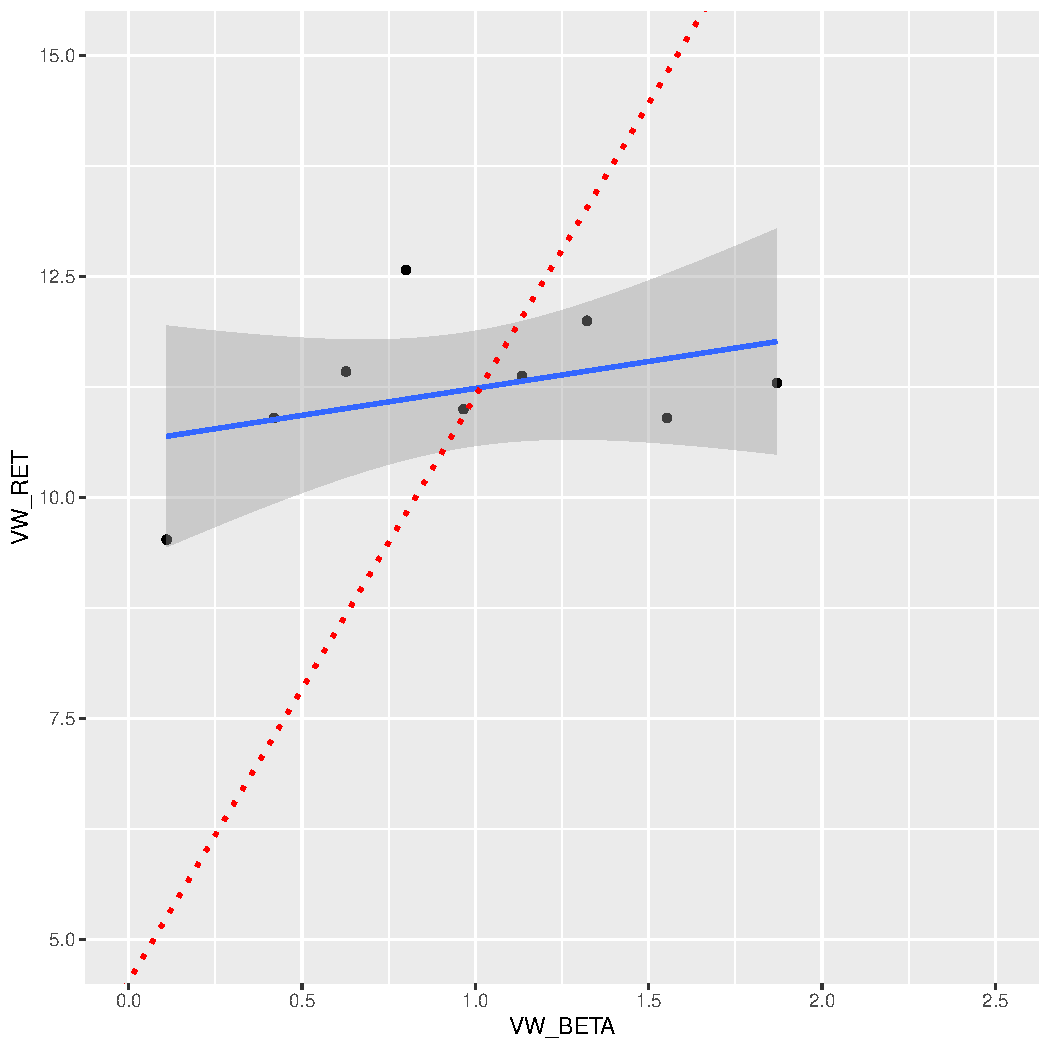
\includegraphics[trim = 0in 0in 0in 0in, 	width=1.75in]{CRSP_COMP_files/figure-latex/capm_vw_36.pdf}}
 \subfigure[60 Months Window]{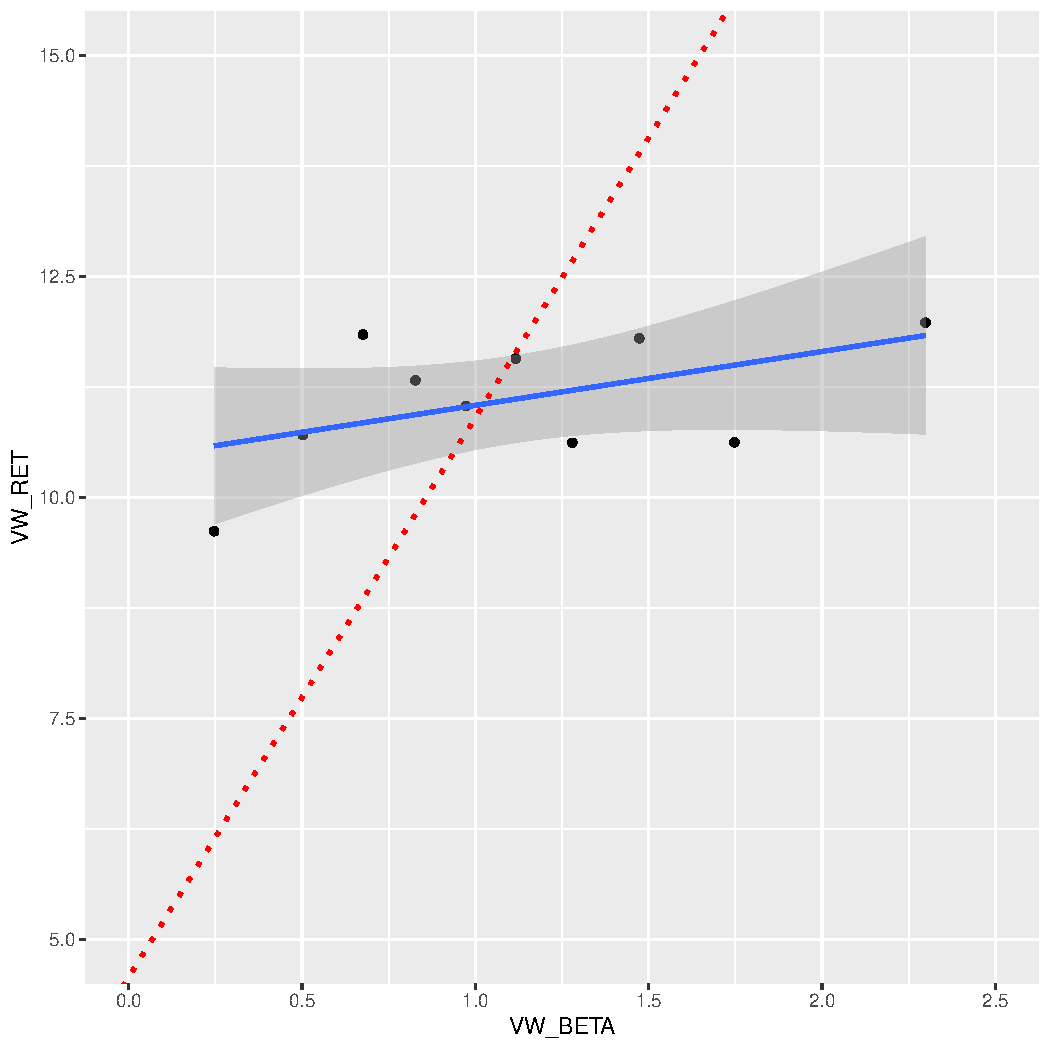
\includegraphics[trim = 0in 0in 0in 0in, 	width=1.75in]{CRSP_COMP_files/figure-latex/capm_vw_60.pdf}} 
 \subfigure[120 Months Window]{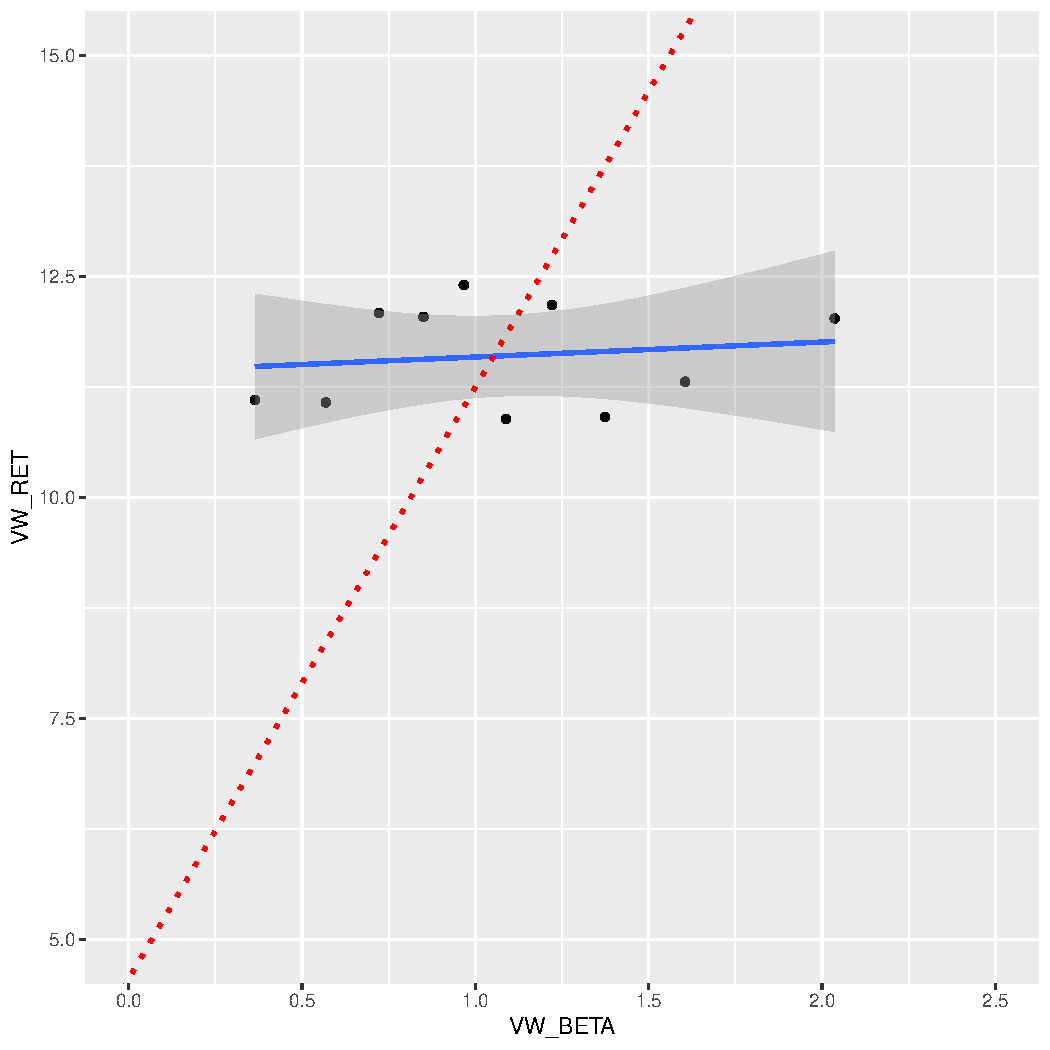
\includegraphics[trim = 0in 0in 0in 0in, 	width=1.75in]{CRSP_COMP_files/figure-latex/capm_vw_120.pdf}} 
 \end{center}
 
 \vspace{-0.25in}
\end{figure}





Consistent with \cite{fama2004capital}, we note that the portfolio results denote a flatter line than the one suggested by the CAPM. At the same time, we note that the results are noisy and sensitive to the sample size choice. In unreported results, we find that the negative relationship suggested by \cite{frazzini2014betting}  is only evident when the betas are estimated using daily returns and portfolios are equally weighted. 



\hypertarget{concluding-remarks}{%
\section{Concluding Remarks}\label{concluding-remarks}}

This article provides a brief illustration of merging the CRSP
(security prices/returns) data with the COMPUSTAT (financial) data. The
illustration is conducted for portfolio formation using
book data. The final result is combining monthly market data with annual
accounting data. However, researchers interested in performing
panel analysis or applying predictive models using machine learning may
prefer merging the data altogether using the same frequency. We leave
this for future research. Nonetheless, we hope this article would
encourage further reproducible empirical asset pricing research while
also helping bridge the gap between the data science
community and the empirical finance literature.


\hypertarget{notes}{%
\section{Notes}\label{notes}}

An html vignette is found on \url{https://rpubs.com/simaan84/CRSP_COMP}.
The Rmd source code can be retrieved using the link.

\bibliography{RJreferences}


\address{%
Majeed Simaan \\
School of Business, Stevens Institute of Technology \\ 
1 Castle Point Terrace, Babbio Center, Hoboken, NJ 07030, USA.\\
}
\href{mailto:msimaan@stevens.edu}{\nolinkurl{msimaan@stevens.edu}}


